\chapter{Nulla-ismeretű protokollok alkalmazása autentikációra}

A nulla-ismeretű protokollok egyik elterjedt alkalmazása a felhasználók autentikálása. Ebben a fejezetben ilyen protokollokat fogunk áttekinteni.

\section{A Schnorr azonosító protokoll}

Ezt megelőzően is léteztek már nulla-ismeretű protokollok, mint Fiat-Shamir \cite{FiatShamir} és annak továbbfejlesztései (FFS \cite{FeigeFiatShamir} és GQ protokollok \cite{GuillouQuisquater}), amelyek biztonságosságukat a faktorizációs probléma nehézségéből nyerik. 

A Schnorr protokoll \cite{Schnorr}, ezekkel ellentétben a diszkrét logaritmus problémából nyeri biztonságosságát. Manapság az elliptikus görbe kriptográfia egyre nagyobb teret nyer, köszönhetően a kisebb kulcsméretnek, vele együtt pedig növekszik az elliptikus görbe diszkrét logaritmus probléma. Ezért úgy érzem előnyösebb Schnorr protokollját áttekinteni, mint az őt megelőző faktorizáción alapuló protokollokat.

\subsection{A diszkrét logaritmus probléma}\cite{BerczesPetho}

\begin{definition}
    Legyen $m$ egy pozitív egész szám. Egy $g$ egész számot primitív gyöknek nevezünk modulo $m$ ha minden $b \in \{1,2,...,m-1\}$ szám esetén, melyre $(b,m) = 1$ létezik olyan $k$ pozitív egész szám, melyre $g^k \equiv b \pmod{m}$.
\end{definition}

\begin{theorem}
    Akkor, és csakis akkor létezik primitív gyök modulo $m$, ha $m = 2$, $m = 4$, $m = p^k$ vagy $m = 2p^k$, ahol $p$ valamely pozitív szám.
\end{theorem}

\begin{definition}
    Legyen $p$ egy pozitív prímszám, $b$ egy egész szám, melyre $(b, p) = 1$, és legyen $g$ egy primitív gyök modulo $p$. Azt a legkisebb pozitív egész $k$ számot, melyre teljesül, hogy $g^k \equiv b \pmod{p})$ a $b$ szám $g$ alapú diszkrét logaritmusának nevezzük modulo $p$.
\end{definition}

Miközben a modulo $p$ történő hatványozás nagy $p$ értékek esetén is gyorsan kiszámítható, addig ennek megfordítása, a diszkrét logaritmus kiszámítása nagyon időigényes feladat.

\subsection{A Schnorr azonosító protokoll algoritmusa}

A protokoll a rendszer paraméterek inicializáló lépésével indul.

\begin{algorithm}[H]
    \floatname{algorithm}{Algoritmus}
    \caption{Rendszer inicializáció}
    \label{algorithm:systemInit}
    \begin{algorithmic}
        \Procedure{sys\_init}{$t$} \Comment $2^{-t}$ a rendszerben a helyes tippelés valószínűsége
        \State $p$ prím inicializálása
        \State $q$ prím inicializálása \Comment $q | p-1$
        \State $\alpha$ elem kiválasztása \Comment $\alpha \in \mathbb{Z}_{p}$ és rendje $q$
        \EndProcedure
    \end{algorithmic}
\end{algorithm}

\begin{algorithm}[H]
    \floatname{algorithm}{Algoritmus}
    \caption{Felhasználói paraméterek generálása}
    \label{algorithm:userInit}
    \begin{algorithmic}
        \Procedure{user\_init}{$I_{A}$} \Comment $I_{A}$ a felhasználó egyedi azonosítója
        \State $s$ privát kulcs generálása \Comment ez egy random szám az $\{1,2,...,q\}$ halmazból
        \State $v = \alpha^{-s} \pmod{p}$ publikus kulcs kiszámítása
        \State $\alpha$ elem kiválasztása \Comment $\alpha \in \mathbb{Z}_{p}$ és rendje $q$
        \State A rendszerrel aláíratja az $(I_{A}, v)$ párost, ezzel előáll $sign_{A}$
        \EndProcedure
    \end{algorithmic}
\end{algorithm}

Az azonosító protokoll-t mutatja a \ref{Figure::SchnorrProt} ábra:

\begin{figure}[H]
    \centering
    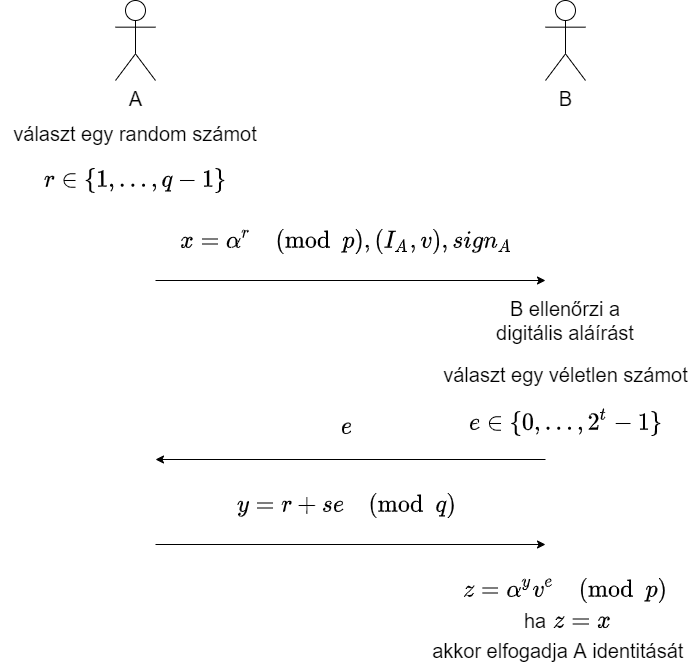
\includegraphics[width=0.6\textwidth]{Schnorr-protokoll.png}
    \caption{Schnorr azonosító protokoll.}
    \label{Figure::SchnorrProt}
\end{figure}

\subsection{A Schnorr azonosító protokoll biztonságossága}

\begin{itemize}
    \item Biztonság: A biztonságosság egyik fő szereplője a $t$, ezt olyan módon kell megválasztani, hogy $2^{-t}$ kellően kicsi legyen, hiszen ez a valószínűsége a helyes tippelésnek a választott $e$ értékre. A másik fontos pontja a protokollnak a megfelelő méretű $q$ választása, mert ez felelős a diszkrét logaritmus probléma nehézségéért.
    \item Helyesség: A protokollt áttekintve, belátható, hogy $s$ ismerete nélkül nem lehetséges senki számára, hogy $A$-nak adja ki magát, mert ezen információ ismeretében képes csak sikeresen végigjátszani a folyamatot.
    \item Nulla-ismeret: A protokoll csak akkor teljesíti a nulla-ismeret tulajdonságot, ha a hitelesítő fél becsületesen jár el. Ez azt jelenti, hogy az $e$ értéket valóban random módon választja ki és nem a kapott $x$ értékétől függően. Ha $x$ értéke alapján választ egy számára megfelelő $e$-t, akkor képes információt kinyerni a felhasználó a bizonyító fél titkával kapcsolatban.
\end{itemize}

\begin{minipage}{\textwidth}
Ezen felül rendkívül fontos követelménye ennek a protokollnak, hogy egy interaktív folyamat során ne használjuk kétszer ugyanazt a random $r$ értéket, hiszen ha kétszer használnánk egyszerűen kiszámíthatóvá válik az $s$ titkunk a következő módon:

$(y_1 - y_2) / (e_1 - e_2) \pmod{q}$ \\
$= (r + se_1) - (r + se_2) / (e_1 - e_2) \pmod{q}$ \\
$= s(e_1 - e_2) / (e_1 - e_2) \pmod{q}$ \\
$= s$
\end{minipage}

\section{M-Pin protokoll}

Az M-Pin protokoll \cite{MPin} egy rendkívül modern elgondolása az autentikációnak, ami a jelenlegi felhasználónév és jelszó alapú rendszerek egy működőképes alternatívája. Ahogy korábban is említettem a jelszavas rendszerek nagy hátránya, hogy a szervereken létezik egy adatbázis amiben a felhasználói jelszavak tárolásra kerülnek többnyire hash-elt változatban (azonban még előfordulnak olyan esetek is, amikor a tényleges jelszót tárolják). Ezeket az adatbázisokat gyakran feltörik és ellopják.

Az M-Pin célja az, hogy a regisztrált felhasználóknak osszunk ki egy nagy kriptográfiai titkot, amelyet felhasználva nulla-ismeretű bizonyítékkal képes igazolni kilétét. Így nincs szükség arra, hogy bármilyen felhasználói titkot tároljon a szolgáltató a szerverein. Erre a módszerre alapozva kínál szolgáltatást a MIRACL\footnote{https://miracl.com/}.

Mielőtt áttekintenénk, hogyan is működik ez az eljárás, fontos ismernünk az elliptikus görbék és a párosítás alapjait.

\subsection{Elliptikus görbe kriptográfia}

A témáról kimerítően a \cite{ECCGuide, ECCHandbook} könyvekben lehet olvasni, én csupán a protokoll megértéséhez szükséges részleteket szeretném áttekinteni.

A kriptográfiában kiemelt szereppel bírnak az úgynevezett Weierstrass elliptikus görbék: $$y^2 = x^3 + ax + b.$$ Egy ilyen görbéről látható példa a \dotref{Figure::ECC::EllipticCurve} ábrán.

\begin{figure}[H]
    \centering
    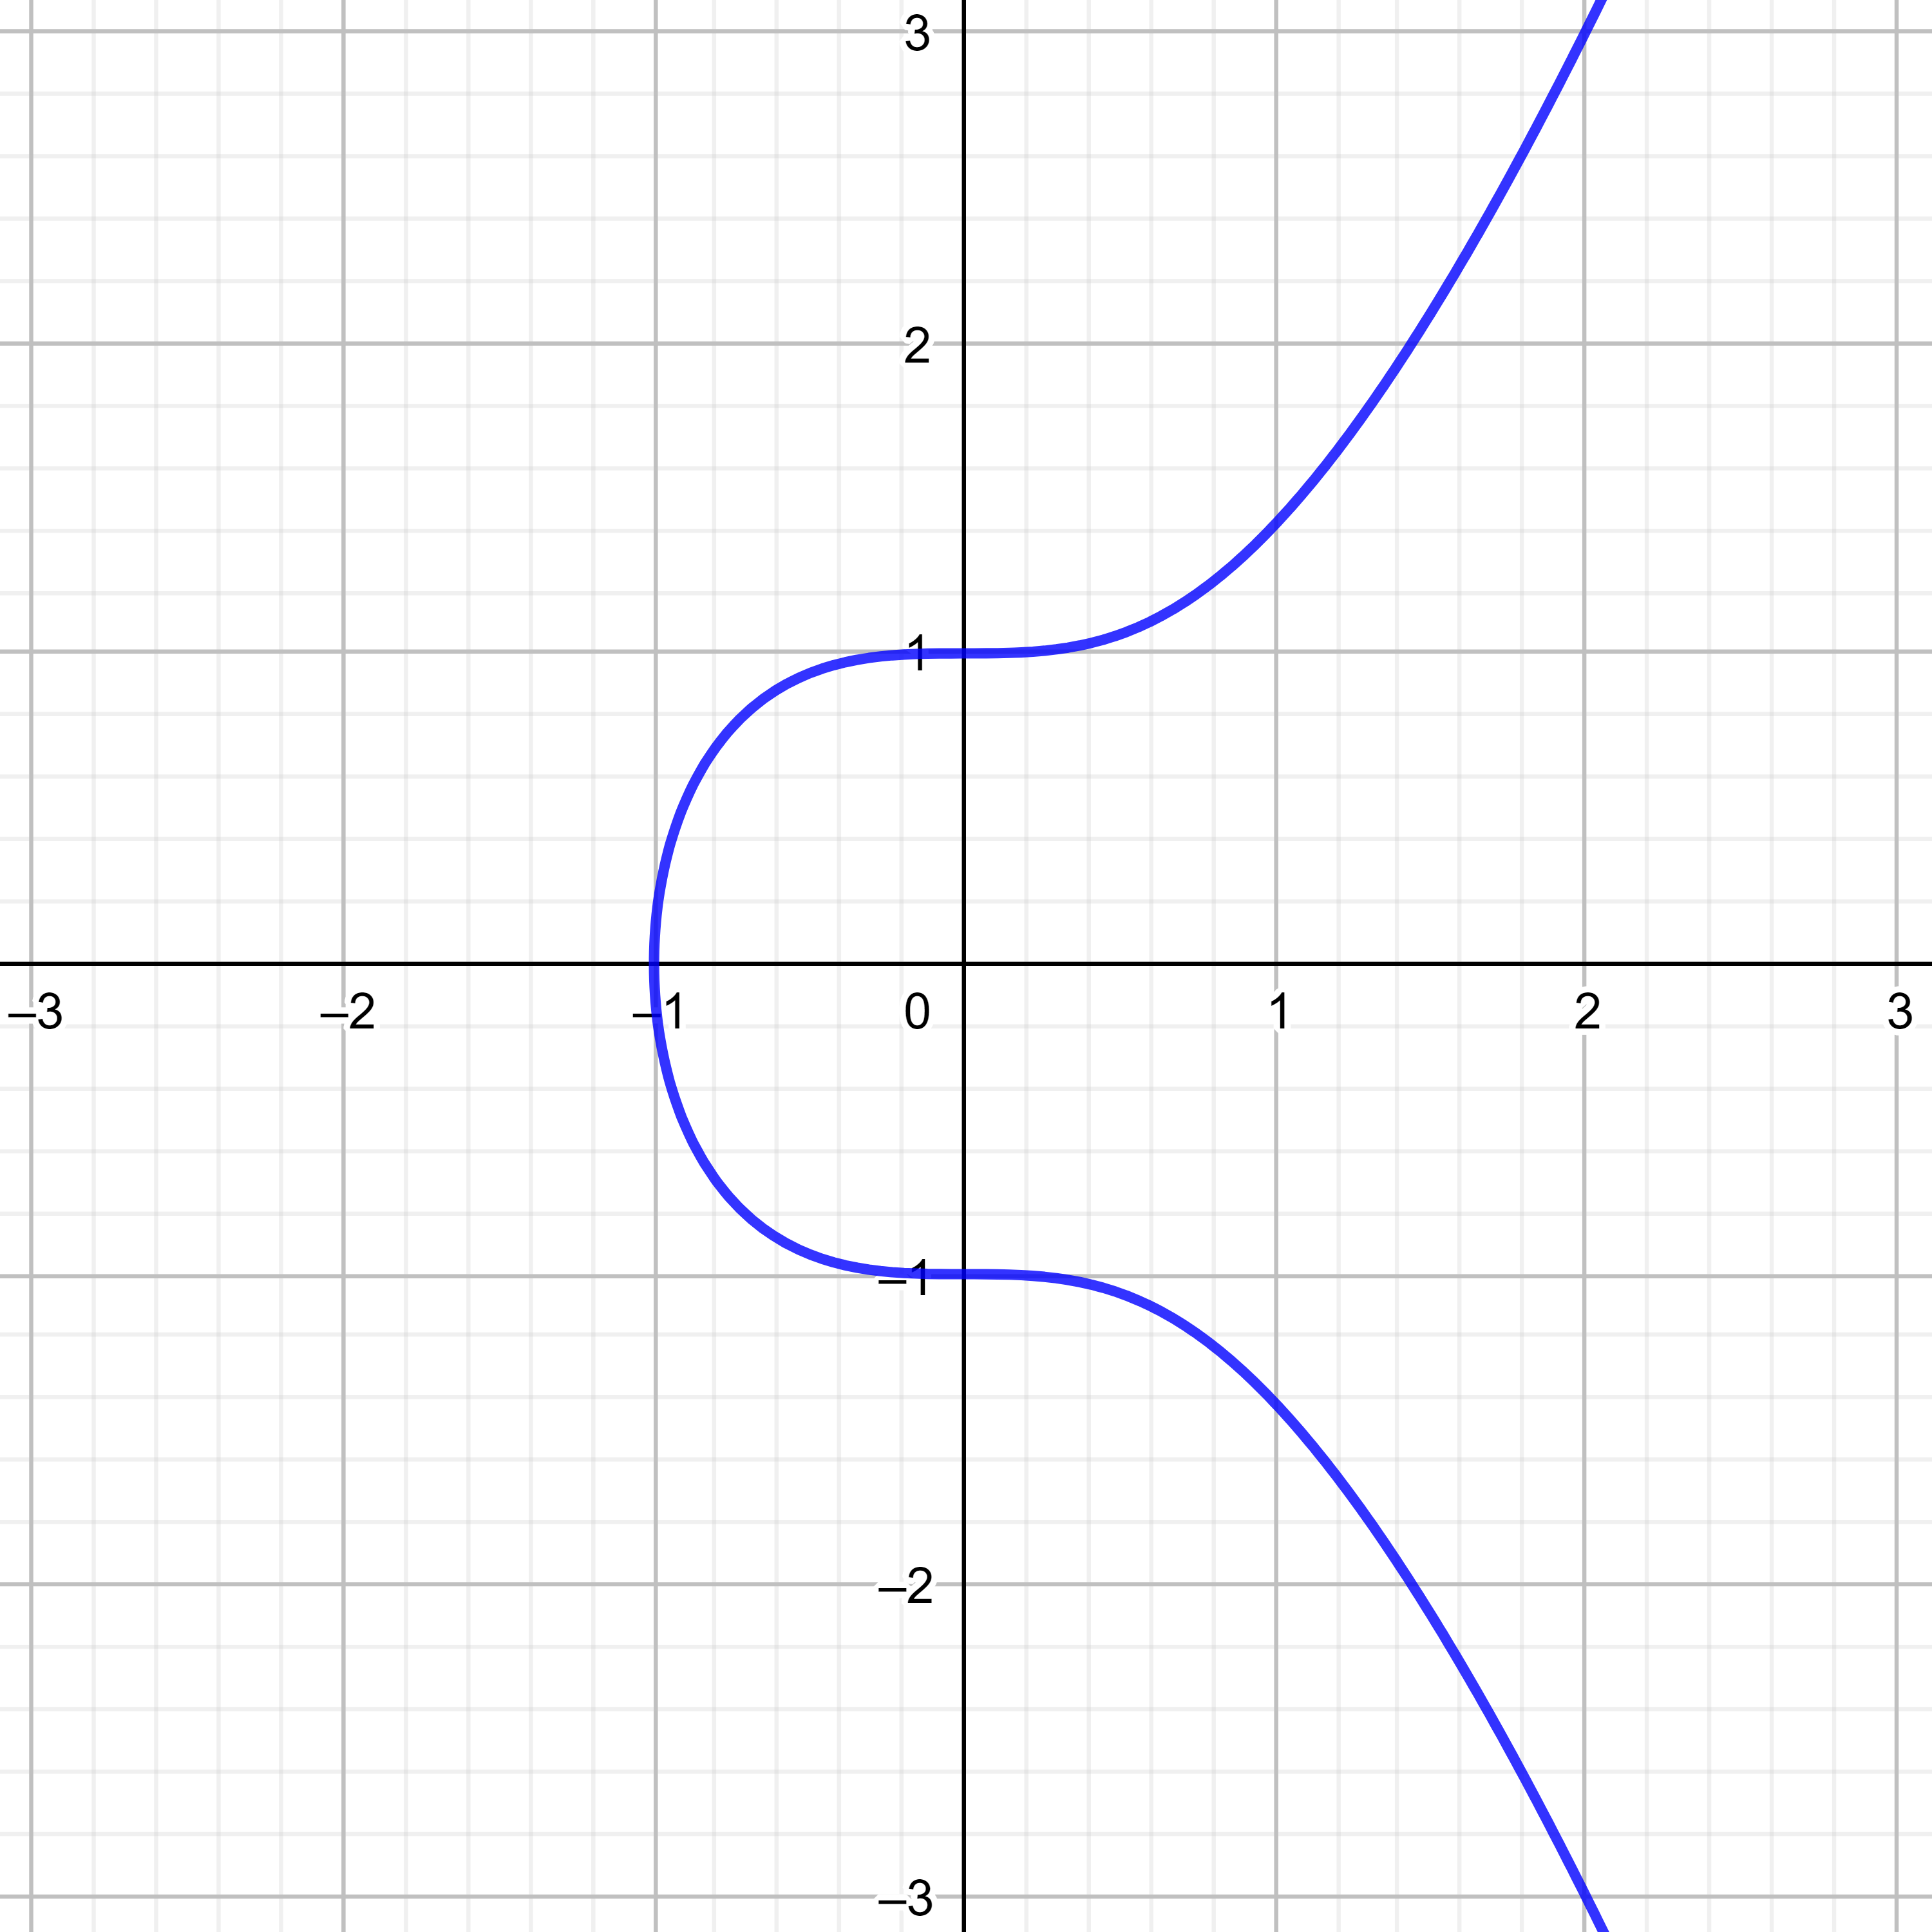
\includegraphics[width=0.4\textwidth]{elliptikus-gorbe.png}
    \caption{Az $y^2 = x^3 + 1$ görbe a valós számok teste felett.}
    \label{Figure::ECC::EllipticCurve}
\end{figure}

\subsubsection{Az $E(K) : y^2 = x^3 + ax + b$ görbe tulajdonságai \protect\footnote{Ha $K$ karakterisztikája nem $2$.}}

\begin{outdentlist}
    \item[]
    \textbf{Egységelem.} $P + O = O + P = P$, minden $P \in E(K)$ esetén.

    \item[]
    \textbf{Ellentettek.} Ha $P = (x, y) \in E(K)$, akkor $(x, y) + (x, -y) = O$. Az $(x, -y)$ pontot $-P$-vel jelöljük és $P$ ellentettjének nevezzük. $-P$ is $E(K)$ egy pontja.

    \item[]
    \textbf{Pontok összeadása.} Legyen $P = (x_1, y_1) \in E(K)$ és $Q = (x_2, y_2) \in E(K)$, úgy hogy $P \neq \pm Q$. Ekkor $P + Q = (x_3, y_3)$, ahol 
    \begin{center}$x_3 = \big(\frac{y_2 - y_1}{x_2 - x_1}\big)^2 - x_1 - x_2$ és $y_3 = \frac{y_2 - y_1}{x_2 - x_1}(x_1 - x_3) - y_1$.\end{center}

    \item[]
    \textbf{Pont duplázás.} Legyen $P = (x_1, y_1) \in E(K)$, úgy hogy $P \neq -P$. Ekkor $2P = (x_3, y_3)$, ahol
    \begin{center}$x_3 = \big(\frac{3x_1^2 + a}{2y_1}\big)^2 - 2x_1$ és $y_3 = \frac{3x_1^2 + a}{2y_1}(x_1 - x_3) - y_1$.\end{center} Ha $P = -P$, akkor $2P = O$.

    \item[]
    \textbf{Pontok skalár szorzása.} Legyen $P \in E(K)$ és $n \in \mathbb{Z}$. Ekkor egy lehetséges módszer a skalár szorzásra a \textit{Double-and-Add} módszer: $$nP = \sum_{i = 0}^{t-1} n_i 2^i(P) = n_0P + 2(n_1P + 2(n_2P + 2(... + 2(n_{t-1}P)...))).$$
\end{outdentlist}

Most, hogy ismerjük a műveleteket, bemutatom a protokoll szempontjából fontos tulajdonságot a disztributivitást az elliptikus görbéken.

Legyenek $n \in \mathbb{Z}$ és $P \in E(K)$, ha $n = n_1 + n_2$, akkor $nP = n_1P + n_2P$. Továbbá, legyen $P_1, P_2 \in E(K)$, ekkor $n(P_1 + P_2) = nP_1 + nP_2$.

Azonban az elliptikus görbe kriptográfia legfontosabb tényezője az elliptikus diszkrét logaritmus probléma, ami egy nehezen megoldható probléma.

\begin{definition*}
    Az \textbf{elliptikus diszkrét logaritmus probléma} (ECDLP): Adott egy $E$ elliptikus görbe az $\mathbb{F}_q$ véges test felett, egy $n$ rendű $P \in E(\mathbb{F}_q)$ pont, valamint egy $Q$ pont, amely $P$ többszöröse. Keressük azt az $l \in [0, n - 1]$ egész számot, amelyre $Q = lP$ teljesül. Ezt a számot a $Q$ pont $P$ alapú elliptikus diszkrét logaritmusának nevezzük.
\end{definition*}

\subsection{Párosítás-alapú kriptográfia}

A párosításról és a kriptográfiában való alkalmazásáról részletes olvasmány a Guide to pairing-based cryptography \cite{PBCGuide}. Számunkra azonban elegendő a párosítás műveletének tulajdonságait ismerni, továbbá azt, hogy a párosítás alkalmazásával komplex matematikai problémákat vagyunk képesek redukálni azzal, hogy egy másik csoportba visszük át a problémát.

Jelöljön $G_1, G_2$ additív, míg $G_\mathbb{T}$ multiplikatív $r$ rendű csoportokat. Az $e$ párosítás egy olyan $e : G_1 \times G_2 \rightarrow G_\mathbb{T}$ leképezés, amely a következő tulajdonágokkal rendelkezik:
\begin{outdentlist}
    \item[] \textbf{Bilineáris.} Jelölje $\mathbb{Z}_r$ az egész számok halmazát modulo $r$, ekkor $\forall P_1 \in G_1, P_2 \in G_2$ és $a, b \in \mathbb{Z}_r$ esetén $e(aP_1, bP_2) = e(P_1, P_2)^{ab}$.

    \item[] \textbf{Nem elfajuló.} Ha $P_1 \neq 0_{G_1}$ és $P_2 \neq 0_{G_2}$, akkor $e(P_1, P_2) \neq 1_{G_\mathbb{T}}$, ahol $0_{G_1}$ (illetve $0_{G_2}$ és $1_{G_\mathbb{T}}$) az egységeleme a $G_1$ csoportnak (illetve $G_2$ és $G_\mathbb{T}$ csoportnak).

    \item[] \textbf{Hatékonyan számítható.}

    \item[] \textbf{Nehezen megfordítható.}
\end{outdentlist}

\subsection{Az M-Pin protokoll algoritmusa}

A protokollban három entitás játszik szerepet. Az első a Megbízható Hatóság (Trusted Authority, innentől TA). Ennek a szerepe, hogy a megfelelő titkos kulcsokat kiossza a második entitásnak, a felhasználóknak és a harmadik entitásnak, a szervereknek (különböző szolgáltatásoknak). 

A TA funkcionalitása nagyon hasonlít az azonosító-alapú (identity-based) protokollok körében alkalmazott Privát Kulcs Generátorra, valamint maga a kulcs generálás folyamata is ugyanaz. A TA rendelkezik egy mesterkulccsal $s$, és a felhasználók valamilyen azonosítókkal $ID$. A felhasználók kulcsának kiszámítása úgy megy végbe, hogy egy $H$ hash függvényt alkalmazva kiszámítjuk $sH(ID)$-t, ezzel előáll egy $G_1$ béli elem. Majd ezt továbbítjuk a felhasználónak. A szerver kulcsának generálása, pedig úgy történik, hogy a szerverhez rendelünk egy egyedi $Q \in G_2$ generátort, majd kiszámítjuk $sQ$-t és azt továbbítjuk.

A TA könnyedén alakítható elosztott rendszerré, csupán az $s$ mesterkulcsot kell tényezőkre bontani, $s = s_1 + s_2$ majd a tényezőkkel külön-külön elvégezni a fenti műveleteket, amiknek eredményét a felhasználó összeadva megkapja a kulcsát. Ezzel egyszerűen biztonságosabbá lehet tenni a rendszert, hisz nem egy helyen lesz tárolva az $s$ mesterkulcs.

A protokoll különlegessége, hogy a kulcs könnyedén szétbontható egy tokenre és egy PIN kódra, ezzel több faktorossá alakítva az autentikáció folyamatát. Legyen a választott PIN kód $\alpha$ és $A = H(ID)$, ekkor a token $(s - \alpha)A$, ami úgy számolható, hogy $sA$-ból kivonjuk $\alpha A$-t. $sA$ visszaállítása pedig a következő módon történik: $sA = (s - \alpha)A + \alpha A$.

Ezek ismeretében tekinthetjük magát az azonosítás folyamatát, ami a \ref{Figure::MPIN} ábrán látható:

\begin{figure}[H]
    \centering
    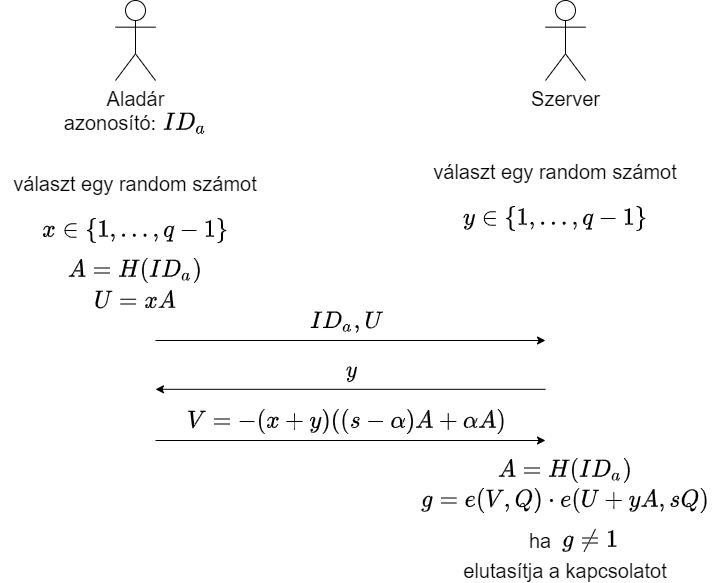
\includegraphics[width=0.5\textwidth]{MPIN.png}
    \caption{M-Pin protokoll.}
    \label{Figure::MPIN}
\end{figure}

\subsection{Az M-Pin protokoll biztonságossága}

\begin{itemize}
    \item Biztonság: A támadási lehetőségek a Diffie-Hellmann problémára és annak variációira vezethetők vissza, amelyek mind nehéz problémák, ezért a protokoll biztonságosnak tekinthető.
    \item Helyesség: A definíció szerinti helyesség olyan szinten nem jelenik meg, hogy a protokoll egyik résztvevője a TA ismeri és bármikor kiszámíthatja a felhasználói titkot. Azonban ettől eltekintve belátható, hogy a felhasználó által választott $\alpha$ PIN kód és a token ismerete nélkül nem végrehajtható a protokoll.
    \item Nulla-ismeret: A szerver nem képes információhoz jutni sem a folyamat során választott $x$ értékről, sem a felhasználói titokról, mert mind a két esetben az ECDLP megoldása szükséges, ami nehéz feladat. Ezért, ha $y$-t nem random módon választja, akkor se képes információt kinyerni.
\end{itemize}